%%%%%%%%%%%%%%%%%%%%%%%%%%%%%%%%%%%%%%%%%%%%%%%%%%%%%%%%%%%%%%%%%%
\section{Smart Grids}
\label{sec:smartgrids}


%According to the IEEE smart grid initiative [1], “the smart grid is a revolutionary undertaking—entailing new communications-and-control capabilities, energy sources, generation models and adherence to cross-jurisdictional regulatory structures”.
%https://smartgrid.ieee.org/about-ieee-smart-grid

%aqui intro smart grids
\cite{repsol}
\cite{impact}


%%%%%%%%%%%%%%%%%%%%%%%%%%%%%%%%%%%%%%%%%%%%%%%%%%%%%%%%%%%%%%%%%%
\subsection{Internet of Energy}
\cite{ioe}




%%%%%%%%%%%%%%%%%%%%%%%%%%%%%%%%%%%%%%%%%%%%%%%%%%%%%%%%%%%%%%%%%%
\subsection{Estructura de una Smart Grid}

Una \gls{sg} está constituida por múltiples elementos diferentes como se puede visualizar en la Figura \ref{fig:estructura_sg}. Cada uno de ellos está dedicado a uno de los procesos principales, que se pueden dividir en generación, distribución y consumo. \cite{smartgrid_overview}

\vspace{0.3cm}

\begin{figure}[h]
  \centering
  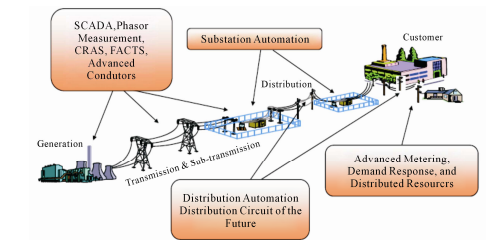
\includegraphics[width=1\textwidth]{img/teoria/estructura_sg.png}
  \caption{Estructura de componentes de una \gls{sg} \cite{smartgrid_overview}}
  \label{fig:estructura_sg}
\end{figure}

\subsubsection{Generación y distribución}

\vspace{3mm}

Dentro del contexto de la generación de energía destacan los sistemas de control y adquisición de datos (del inglés \gls{scada}) \cite{scada}. Estos pueden ser instalados en generadores, como son paneles solares fotovoltaicos o turbinas eólicas, consiguiendo una monitorización remota de los mismos. Mediante la información recopilada a tiempo real permiten conocer los niveles de generación y establecer una predicción de la disponibilidad energética que habrá en el sistema o en un área determinada del mismo.

\vspace{3mm}

Otro dispositivo importante en el campo de la generación y de la distribución energética es la Unidad de Medición de Fasores (del inglés \gls{pmu}). Se emplea para medir con una alta precisión los fasores de tensión y corriente en la red eléctrica, proporcionando información relevante sobre las magnitudes y fases de las ondas sinusoidales. Debe contar con una alta tasa de muestreo para capturar eventos transitorios o cambios rápidos en la red y, en consecuencia, tener la capacidad de identificar o detectar a tiempo real posibles anomalías que se puedan dar en la distribución. Es por ello que, el \gls{pmu} se trata de un componente imprescindible para comprobar y garantizar la estabilidad de la \gls{sg}. %BIB

\vspace{3mm}

La confiabilidad y la seguridad de la red también reside en los Sistemas de Transmisión de Corriente Alterna Flexibles (del inglés \gls{facts}) \cite{facts}. Estos vienen dados por la necesidad de superar las limitaciones técnicas introducidas por las redes eléctricas, como son las térmicas o las respectivas al voltaje. En otros términos, incrementan la potencia transmitida y aportan flexibilidad al permitir modificar de forma dinámica los parámetros eléctricos ante cambios en la configuración de la red. 

\vspace{3mm}

Los \gls{facts} incluyen todos los elementos electrónicos basados en tecnología de alta potencia y que son empleados dentro de una \gls{sg} para la transferencia de energía de CA y el control de la potencia reactiva. También, realizan tareas de reducción de impedancia en las líneas de transmisión y de optimización del factor de potencia y pueden actuar tanto a nivel individual como de forma coordinada con otros controladores.

\vspace{3mm}

La primera generación de \gls{facts} emplea interruptores controlados por tiristores, mientras que la segunda tiene como base convertidores estáticos de conmutación. En la Tabla \ref{tab:facts} se visualizan las tecnologías \gls{facts} más relevantes. \cite{facts2}

\vspace{3mm}

\begin{table}[!h]
    \centering
    \resizebox{\textwidth}{!}{
    \begin{tabular}{| c | c | m{6cm} |}
    \hline
    \rowcolor[HTML]{EFEFEF}
    Generación & Tipo & \multicolumn{1}{c|}{Descripción} \\ \hline
    \multirow{2}{*}{1º} 

    & \gls{tcsc} & Controla el flujo de potencia tanto reactiva como activa por la línea de transmisión mediante el ajuste de impedancia en serie y amortigua las oscilaciones.
    
    \\ \cline{2-3}

    & \gls{svc} & Absorbe o suministra potencia reactiva según las necesidades de una línea de transmisión a través de la variación de la susceptancia en paralelo. Ayuda a mantener el voltaje estable en la red.

    \\ \hline
    \multirow{4}{*}{2º} 
    
    & \gls{statcom} & Compensa la potencia reactiva al igual que el \gls{svc}, pero en este caso empleando electrónica de potencia para proporcionar una respuesta más rápida.

    \\ \cline{2-3} 

    & \gls{upfc} & Combina las funciones de un \gls{tcsc} y un \gls{svc}, teniendo la capacidad de controlar en una línea de transmisión tanto la impedancia en serie como la susceptancia en paralelo.

    \\ \cline{2-3} 

    & \gls{sssc} & Modifica dinámicamente la impedancia y es capaz de controlar la fase y la amplitud de la tensión en la línea.

    \\ \cline{2-3} 

    & \gls{ipfc} & Conecta varias líneas de transmisión en paralelo. No obstante, modula la impedancia y la fase de la tensión de cada línea de transmisión de forma independiente, lo que permite operar sobre el flujo de potencia de una forma controlada. Mejora la capacidad de transmisión y reduce las pérdidas energéticas. 
    
    \\ \hline
    \end{tabular}
    }
    \caption{Tecnologías FACTS de 1ª y 2ª generación}
    \label{tab:facts}
\end{table}

\subsubsection{Consumo}

Poniendo el foco en el consumo, es imprescindible conocer la cantidad de energía demandada por los clientes que pertenecen a una \gls{sg}. La instalación de sensores o medidores inteligentes (del ingles \textit{smart meters}) en las viviendas o ubicaciones finales posibilitan el registro constante de datos respectivos al consumo de energía, niveles de voltaje, corriente y factor de potencia. Estos son almacenados, analizados y procesados por las distribuidoras de energía para obtener a partir de los mismos la información necesaria sobre el comportamiento de los usuarios. \cite{stab}

\vspace{3mm}

La gestión de los sensores finales en las \gls{sg}s se caracteriza por su alta complejidad, debido a los grandes volúmenes de datos a manejar. 



% Many benefits can be obtained
% from implementing such technology in the areas of asset management,
% operations planning, monitoring voltage instability, stability margin
% prediction and fault detection.

% Accordingly, many challenges are associated with such implementation; the main issues are related to data
% uncertainty, data quality, data security, and data complexity.




%\subsection{Diferencias respecto a Red convencional}
%Performance in conventional grids and smart grids varies a lot in the sense of both production and consumption. In conventional grids, production is always constant no matter what the consumption is, meanwhile in smart grids, if consumption decreases, this decrease is read and responded to with a decrease in production with the goal of conserving and better distributing power to the rest of the grid. Below are Figures 1 and 2 demonstrating a short comparison between the production and consumption in both conventional power grids and smart grids.









